\section*{Air vehicle} \label{sec:vehicle}

\subsection*{Propulsion and lift system} \label{subsec:vehicle-proplift}

Our air vehicle, shown in Figure \ref{fig:propulsion-system}, is an improved iteration of our previous vehicles, being a X configuration quadrotor with a 500-millimeter frame (diagonally) providing great structural simplicity and stability as well as easy mounting of all necessary sensors due to its large surface area. Its 191-gram carbon fiber sandwich panel makes it very light while providing good structural rigidity as a result of the greater statical moment of area. The 12”x4.5 tri-blade folding propellers, 45~mm diameter Turnigy Multistar 4010-580 brushless motors, 30~A Hobbywing ESCs, and 8,000~mAh 4S 45~90C Turnigy lithium polymer batteries can generate a total of 5500 g of thrust, thus accommodating payloads from 2.5~kg up to 3~kg at 50~\% thrust with usual flight times of about 11 to 13 minutes.

\begin{figure}[h]
	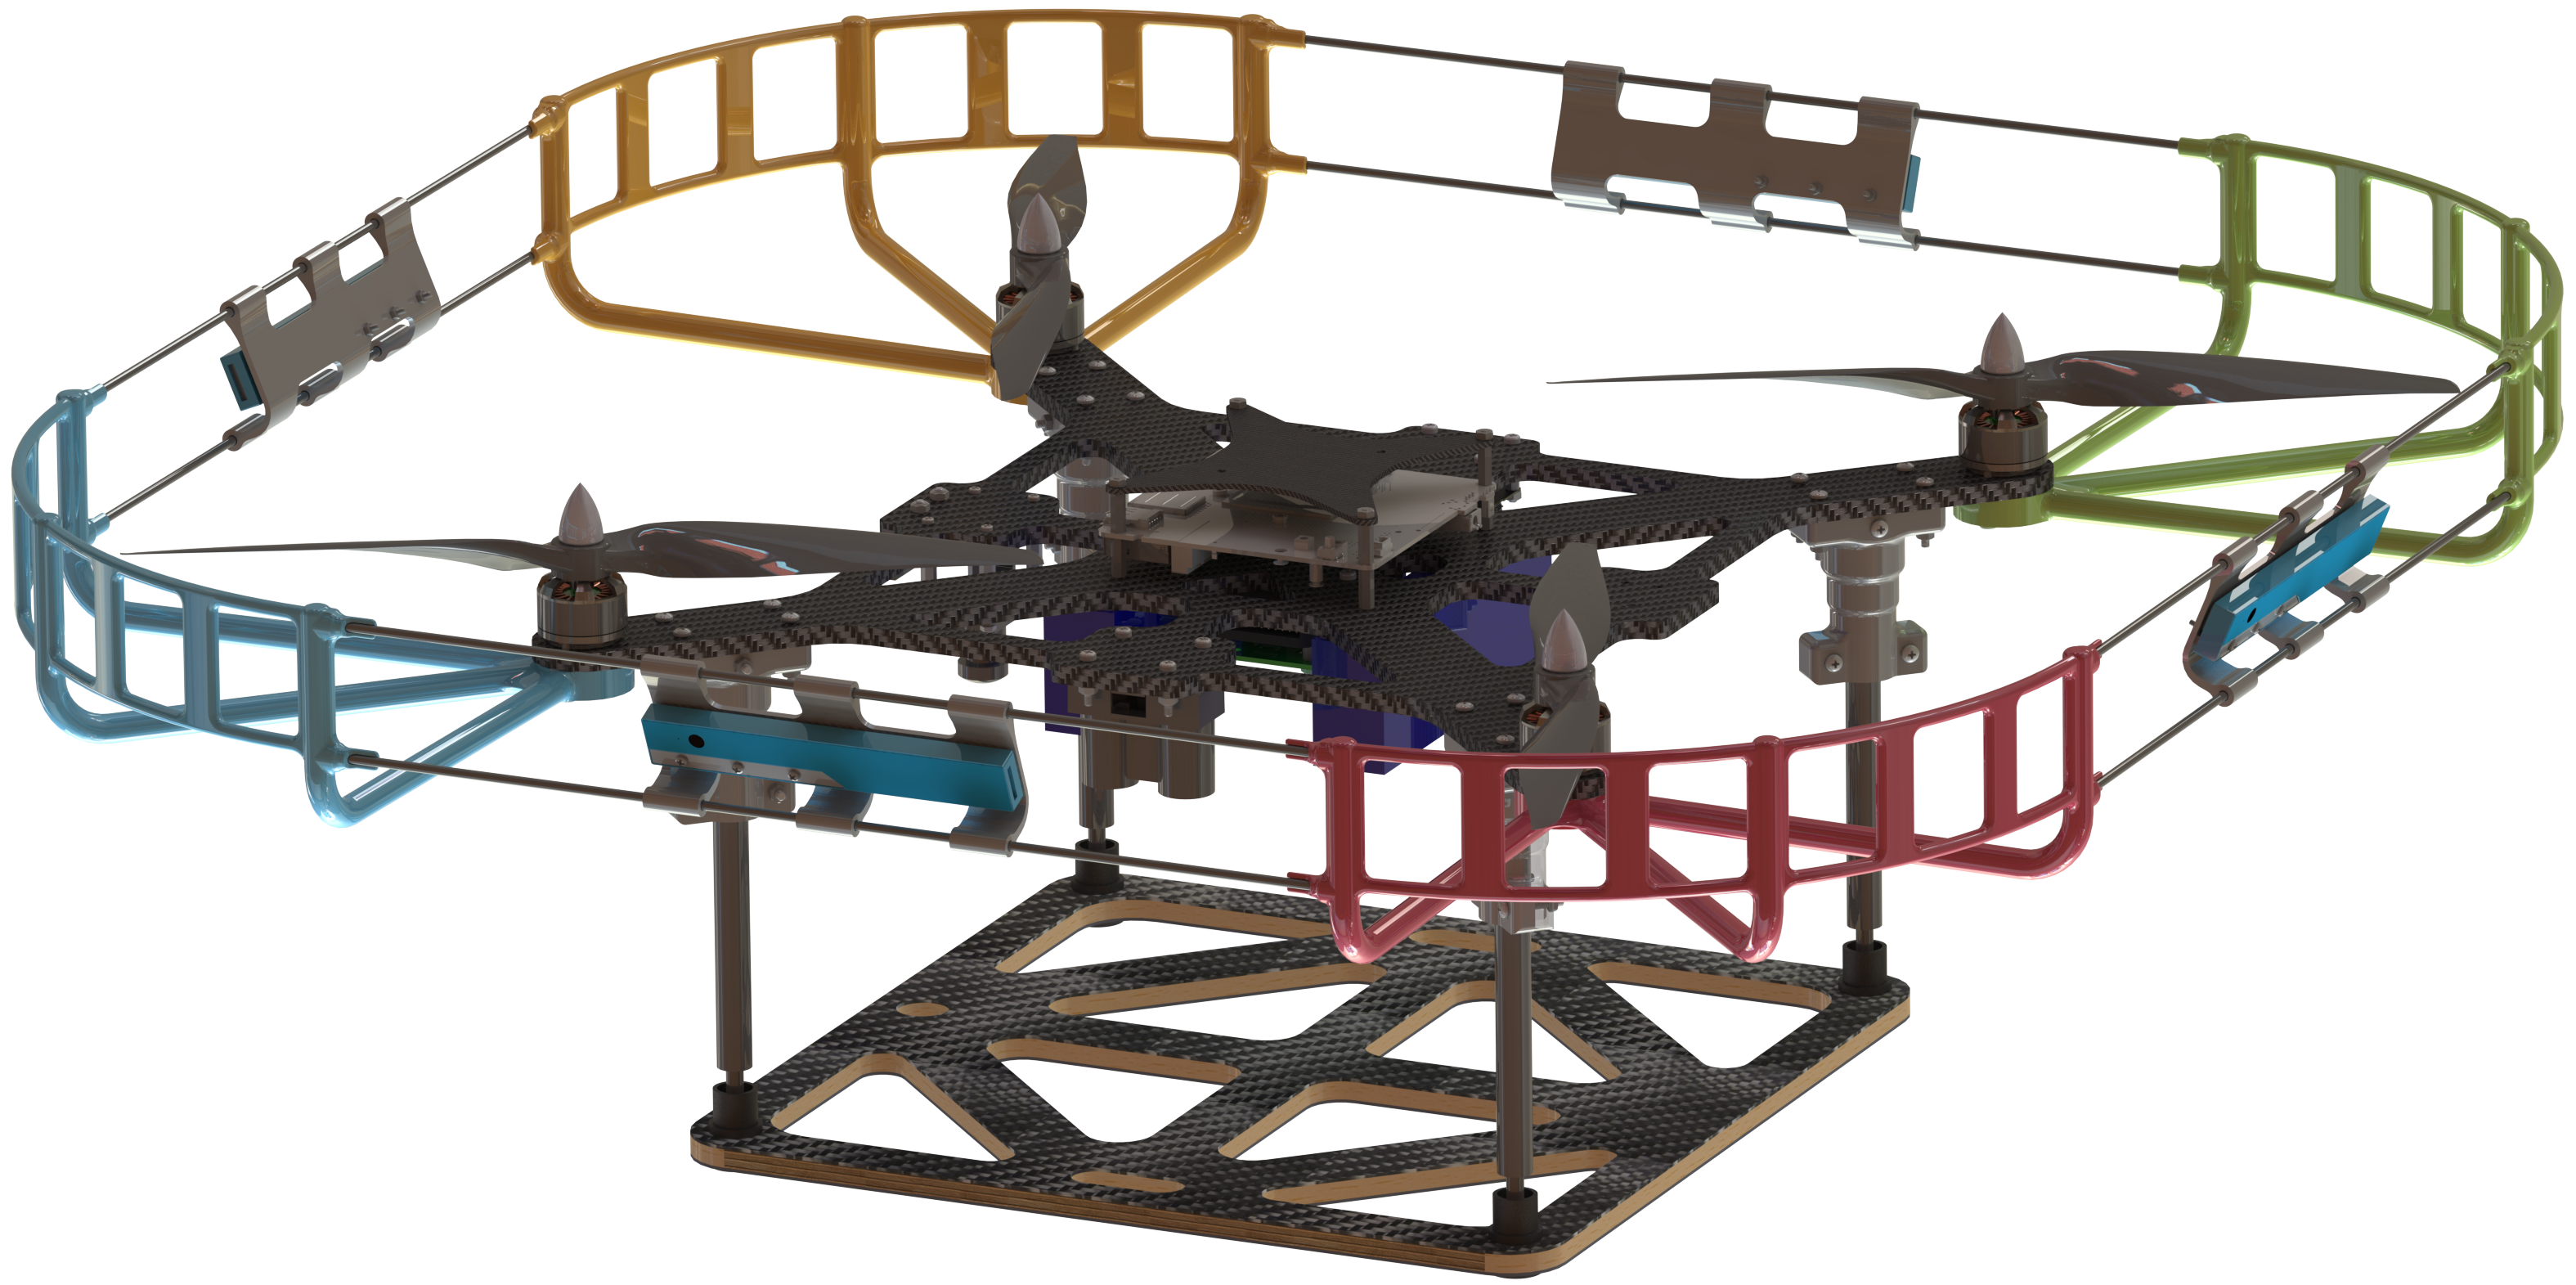
\includegraphics[width=0.8\textwidth]{render_quad_2.png}
	\vspace{-0.3cm}
	\caption{Propulsion and lift system.}
	\label{fig:propulsion-system}
\end{figure}


\subsection*{Guidance, navigation, and control} \label{subsec:vehicle-gnc}

\subsubsection*{Stability augmentation system}

Our vision localization system is based on feature tracking of the arena’s grid and thereby produces a position and yaw estimate of the vehicle’s state. This estimate is then used in the FCU’s position estimate as explained in the Control System Architecture section. The procedure goes as follows.

\vspace{-0.5cm}
\begin{enumerate} \itemsep -4pt
	\item \textit{Intersection Detection} In order to detect the line intersections, the image’s perspective is removed, and the white lines are detected with the Canny algorithm \cite{canny1986computational} and merged based on their position and angle. The intersections are then trivial to detect.
	\item \textit{Pose calculation} Calculate the camera’s pose relative to the intersections using the \textit{PnPRANSAC} algorithm available in \textit{OpenCV} \cite{lepetit2009epnp}.
	\item \textit{Prediction} The points positions are predicted based on the vehicle’s estimated state i.e. its pose, orientation and linear acceleration. The prediction is generated using an unscented Kalman filter. The filter also integrates data from other sensors (e.g. the IMU) in order to make it more reliable.
	\item \textit{Matching} The points and their predictions are matched, based on the smallest euclidean distance.
	\item \textit{FCU communication} Calculate the absolute position of the drone and send it to the FCU. At the same time, the calculated position is used to refine the prediction of the next set of points.
\end{enumerate}

\subsubsection*{Navigation}

Figure \ref{fig:gnc-software} presents the navigation pipeline for the path planning. The first modules are dedicated to targets detection and tracking to provide accurate information about the state of the ground robots in a way that the decision making module can determine which target trajectory needs to be modified. 

\begin{figure}[h]
	\includegraphics[width=\textwidth]{software_architecture.pdf}
	\vspace{-0.5cm}
	\caption{Software architecture.}
	\label{fig:gnc-software}
\end{figure}

\subsubsection*{Target detection}

There are three layers in the target identification process, as shown in Figure \ref{fig:gnc-detection}. Each of them improves the certainty of a detection. 

The first layer consists of color blob detection using HSV filters included in OpenCV to extract the colors of the target robots (red and green) in the images captured by the cameras. Blur, dilations and erosions are applied to the image to filter the results by reducing noise. Since this technique demands a very accurate color calibration, a remote calibration tool was created for the cameras that will be used prior to our performance to adjust to the environment’s lighting. The results are then passed to the second layer.

The second layer is a blob shape detection. It compares the first layer extracted blobs’ shapes to the known rectangular target’s shape to reduce false positive detections. The shape of the detected blobs is estimated using the “Structural Analysis and Shape Descriptor” \cite{journals/cvgip/SuzukiA85} algorithms available in the OpenCV library. 

The third layer, which is not related to the first two layers, is a circle detection. It is performed into a grayscale image using a circle Hough Transform \cite{yuen1990comparative} available in OpenCV computer vision library. The results are compared with the second layer’s filtered results to improve the certainty of a detected target. Since the camera footage has perspective in it, we used OpenCV’s perspective removal tools to remove that perspective to make the Hough Circle Transform algorithm effective. 

The found circles’ positions are then compared to the second layer’s detected targets and the matching results are then output to other systems.  Figure \ref{fig:gnc-detection} presents a schematization of the detection pipeline.

\begin{figure}[h!]
	\includegraphics[width=\textwidth]{target_detection.pdf}
	\vspace{-0.5cm}
	\caption{Target detection pipeline.}
	\label{fig:gnc-detection}
\end{figure}

\subsubsection*{Target tracking}

The main idea behind this module is that an invisible target must not be non-existent and without any level of priority to the eye of the decision maker module. Therefore, we estimate the position of the hidden robots by using simple Kalman Filters. We use the classical 2D filter for each of the targets. Of course, with time passing, the accuracy of the tracking can drastically drop since the ground robots are moving according to an almost random pattern. However, we suppose that the relatively small arena will make it possible to track quite well even then, because a simple run back and forth can allow the drone to update quite quickly the robots’ tracking data. 

\subsubsection*{Decision making}

Three different strategies are implemented : Target Research, Aggressive and Preventive. In the Target Research strategy, the UAV will hold its altitude and follow the ground robot with the highest priority. The two others strategies are focused on interaction with ground robots and mission completion. The difference between them is that the aggressive one will lead the ground robots toward the green line and the preventive one will avoid any ground robot to cross the red lines. Once the target is chosen, the decision making module will switch between different behaviors based on different factors such as the positions of the selected target, the UAV itself and the desired outcome. Those behaviors can be, for example, following the target or interacting with the robot using the front side bumper or the top touch paddle. A setpoint is finally produced and sent to the obstacle avoidance module.

\subsubsection*{Obstacle avoidance}

To avoid any collision with the obstacle robots we use three Intel Realsense R200 stereo cameras positioned on the front, left and right sides of the UAV. The Intel Realsense R200 infrared stereo sensor has a range of 3 to 4 meters indoor. We use the MoveIt! package \cite{chitta2012ros}, originally designed for manipulator robots to perform three dimensional obstacle avoidance. Many modifications were needed to adapt this path planner to a UAV with 6 degrees of freedom. This package can be adapted to any kind of 3D sensor. Through this path planning approach, our threat avoidance system is more preventive than reactive and thus can find the optimal path between two points and reduce the needed time to complete the mission. Also, unlike a two dimensional approach, the use of stereo cameras solves the fully 3D threat avoidance problem that we will face during the part b of mission 7 when two drones will fly at the same time. When the path is correctly generated, the trajectory execution module follows it by sending the intermediate positions to the PX4 autopilot through the MAVROS interface. 

\subsubsection*{Target interaction}

As the vehicle approach the ground, the multiple sensors become unusable, including the PX4Flow and the stereo cameras. Thus, we implemented a small module that allows us to bypass the obstacle avoidance with the help of preprogrammed sequences that will take over when interacting with ground robots. Some crucial aspects of the environment had to be taken into consideration, including the targets and obstacles movements, both of those being out of reach from our sensors. Moreover, we have to be careful about the drone unpredictable moves when flying at low altitude, as safety comes first when compared to the success of the interaction. Finally, the transition between this blinded mode and the normal decision maker module has to be smooth as some delicate operations cannot be interrupted.

\subsubsection*{Control system architecture}

As explained above and shown in Figure \ref{fig:gnc-controlsystem}, our vision-based pose estimation is used to feed the Local Position Estimator (LPE) included in the PX4 flight stack \cite{feng2016research}. This sensor fusion also uses the LIDAR-Lite for altitude measure, the PX4Flow optical flow as well as IMU data, all of those being either connected or embedded on the Pixhawk flight controller. The estimated position is then returned to the software system through the TF package \cite{foote2013tf} in ROS designed for coordinate frames tracking via MAVROS. Then, the decision making, obstacle avoidance and trajectory execution modules can use the position of the quadrotor to perform their computation. The position estimate is also used by the control system (position then attitude control) to manage properly the motors.

\begin{figure}[h]
	\includegraphics[width=\textwidth]{control_system_architecture.pdf}
	\vspace{-0.5cm}
	\caption{Control system architecture.}
	\label{fig:gnc-controlsystem}
\end{figure}

\subsection*{Flight termination system} \label{subsec:vehicle-killswitch}

The flight termination system, commonly called kill switch, simply cuts off the positive voltage to the propulsion system, since cutting the ground, as proposed in the reference design, caused instabilities with other components on the quadcopter. It does not cut power to the onboard computer to avoid restarting it every time and possibly corrupting data.

The kill switch module is controlled by a RF module which was made on a different board, in order to easily change it without modifying the whole design of the kill switch. This RF module is connected to a receiver which is linked to the kill switch transmitter.
